\section{Missing Transverse Momentum}
\label{sec:reco:MET}

\indent Stable or metastable particles which only interact via the weak force and gravity cannot be directly detected at ATLAS.  In SM, these particles correspond to neutrinos.  In BSM models, there maybe many other weakly interacting particles including WIMPs, gravitons, and a stable neutral SUSY LSP. \\

\indent The presence of weakly interacting particles is inferred through conservation of transverse momentum.  The total transverse momentum is zero in the initial colliding partons at the LHC.  Therefore, any momentum imbalance in the transverse plane must be due to undetected particles in the final state.  \\

\subsection{$\met$ Reconstruction}
\label{sec:MET:reco}

\indent We reconstruct the $\met$ according to equation \ref{eqn:metReco}.  The first term is a negative vector sum of all hard fully calibrated objects and the second term represents the $\vec{E}_t$ of all soft objects in the interaction.  \\

\begin{equation}
\met = - ( \sum_{hard~objects} E_T + \sum_{soft} E_T ) 
\label{eqn:metReco}
\end{equation}

\indent Fully calibrated hard objects include muons, electrons, photons and jets that satisfy their respective {\tt Baseline} selections.  {\tt Baseline} selections applies a loose set of $\pt$ and quality requirements to ensure well reconstructed objects.  {\tt Baseline} object definitions can be found in chapter \ref{chap:objects}. \\

\indent Hadronic taus are not independently reconstructed and calibrated.  Therefore, hadronic taus will most likely be reconstructed as hadronic jets for our analysis.  An overlap removal algorithm have been applied to the {\tt Baseline} objects to remove any potential duplicate objects. \\

\indent We use a track based method called Track Soft Term (TST) \cite{METReco} to reconstruct the contribution from soft objects.  TST build the $\met$ that is not associated with any hard objects by summing the $\pt$ of ID tracks. \\

\indent TST has the advantage of being relatively robust against pileup interactions because TST use ID tracks that are matched with the primary vertex. However TST cannot measure the contribution to $E_T$ from neutral particles because neutral particles do not leave tracks in the ID.  TST is the standard method of estimating $\met$ at ATLAS in Run 2 due to the high pileup conditions. \\

\indent  Only tracks with $\pt > 400 \mev$ are accepted and a number of track quality requirements are applied.  The track quality requirement follows recommendations from the ATLAS tracking performance group and include a minimum of $7$ silicon hits and a requirement on the track $d_0$.  Any tracks within a $\Delta R$ of 0.05 of any electron or photon cluster, the ID tracks of muons, and any ID tracks matched to jets are removed to avoid double counting.  Further details on TST can be found in \cite{METReco}.  \\

\indent $\met$ reconstructed using this method is the standard $\met$ used throughout all signal, control and validation regions in this analysis and is simply referred to as $\met$.  This method of reconstructing $\met$ is also referred to as TST $\met$ to distinguish it from an alternative method of reconstructed $\met$ called track $\met$ described in section \ref{sec:reco:trkMET}. \\

\subsection{Track $\met$ Reconstruction}
\label{sec:reco:trkMET}

\indent Track $\met$ ($\mettrk$) forms a complementary method of reconstructing missing transverse energy.  $\mettrk$, defined in equation \ref{eqn:mettrkReco}, is reconstructed using a negative vector sum of all accepted ID tracks.  \\

\begin{equation}
\mettrk = - \sum_{ID tracks} \pt  
\label{eqn:mettrkReco}
\end{equation}

\indent ID tracks must pass the same requirements described in section \ref{sec:MET:reco} for the TST but no attempt is made at removing tracks that are associated with hard objects.  The one exception to this is tracks associated with an electron.  Because of the high number of interaction expected between an electron and the material in the ID, electron tracks are replaced with the electron calorimeter cluster instead.  \\

\indent Track $\met$ is very robust against pileup conditions ATLAS has very good vertex resolution but neglects the presence of neutral particles.  Track $\met$ is also limited by $\eta$ coverage of the ID which only extends to an $|\eta| < 2.5$.  We use track $\met$ as a cross check on the object based $\met$ reconstruction described in \ref{sec:MET:reco}. Both object based and track based $\met$ must agree loosely in direction for our analysis.  \\

\subsection{$\met$ Performance}
\label{sec:reco:METPerform}

\indent $\met$ performance maybe measured using a number of processes include $Z\rightarrow ll$, $W\rightarrow l\nu$ and ttbar.  $Z\rightarrow ll$ produced with additional jets is considered the gold standard.  Very little intrinsic $\met$ is produced in the $Z\rightarrow ll$ plus jets process.  This presents a good opportunity to study the effect of the $\met$ soft term calculation since no hard invisible particles exist.  The only variable intrinsic to $\met$ reconstruction is the soft term.  All other terms in $\met$ reconstruction depend directly on the resolution of the respective reconstructed hard objects.  $W\rightarrow l\nu$ is also used to study a topology with a high-$\pt$ neutrino and therefore intrinsic $\met$ and ttbar is used to study topologies with a large number of jets. \\

\indent Results from $Z\rightarrow ll$ performance study \cite{METReco} will be summarized here.  The $W\rightarrow l\nu$ $\met$ and ttbar study will not be covered here but further detail can be found in \cite{METReco}. \\

\indent $Z\rightarrow \mu\mu$ events are selected by requiring exactly two same flavor, opposite signed muons with $\pt > 25 \gev$. The dilepton invariant mass must be within $25 \gev$ of the $Z$ mass. \\
%\indent $W\rightarrow e\nu$ events are selected by requiring exactly one electron in the event.  The electron must have $\pt > 17 \gev$.  The TST $\met$ must be greater then $25 \gev$ and the reconstructed transverse mass must be consistent with a $W$ boson decay at greater then $50 \gev$.\\

\indent Distribution of the $\met$ resolution in $Z\rightarrow \mu\mu$ events , defined as the root-mean-squared (RMS) of the $\met$ distribution is shown in figure \ref{fig:MET_reso}.  The $\met$ resolution degrades both with the total amount of $E_T$ in the event and the number of reconstructed vertexes.\\

\begin{figure}[htb]
  \begin{center}
    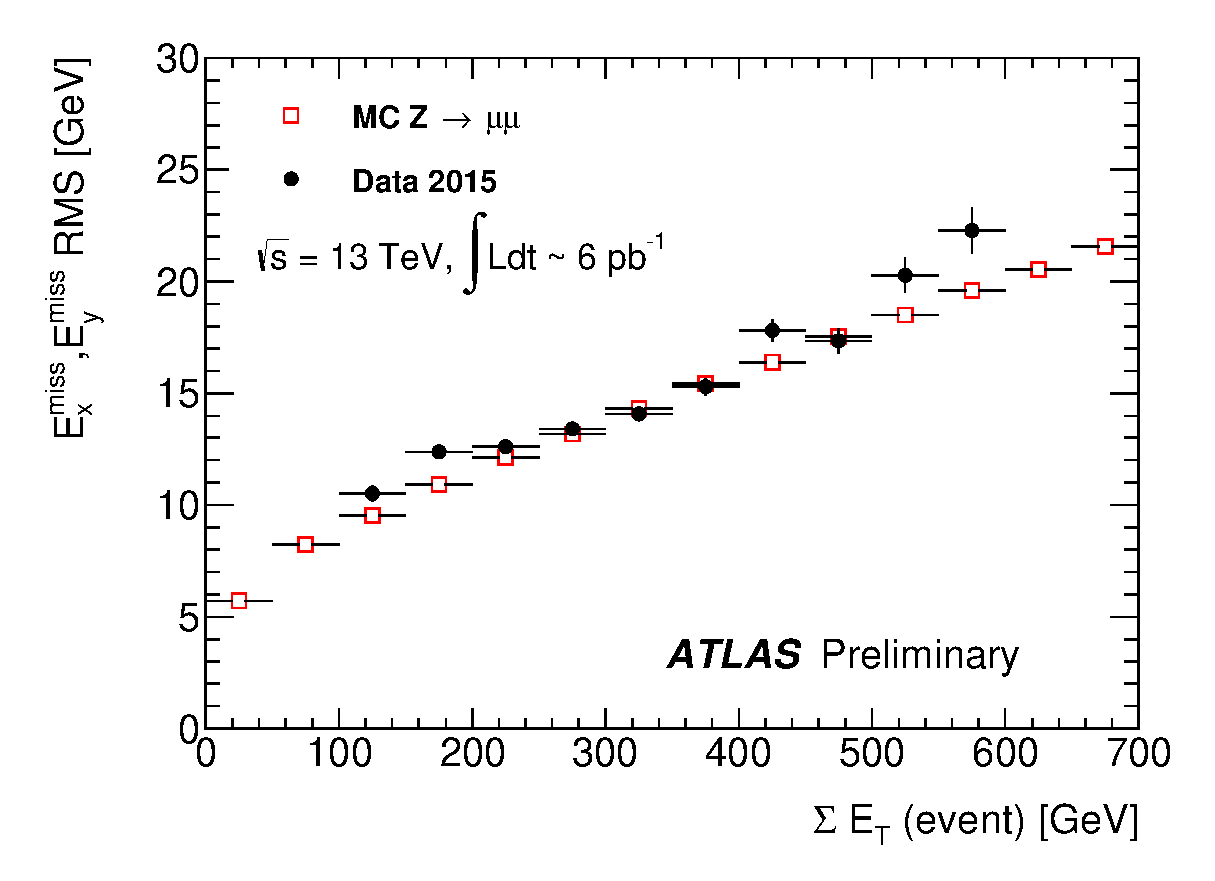
\includegraphics[width=0.45\textwidth]{figures/METCalib/METReso_Et.eps}\hspace{0.05\textwidth}
    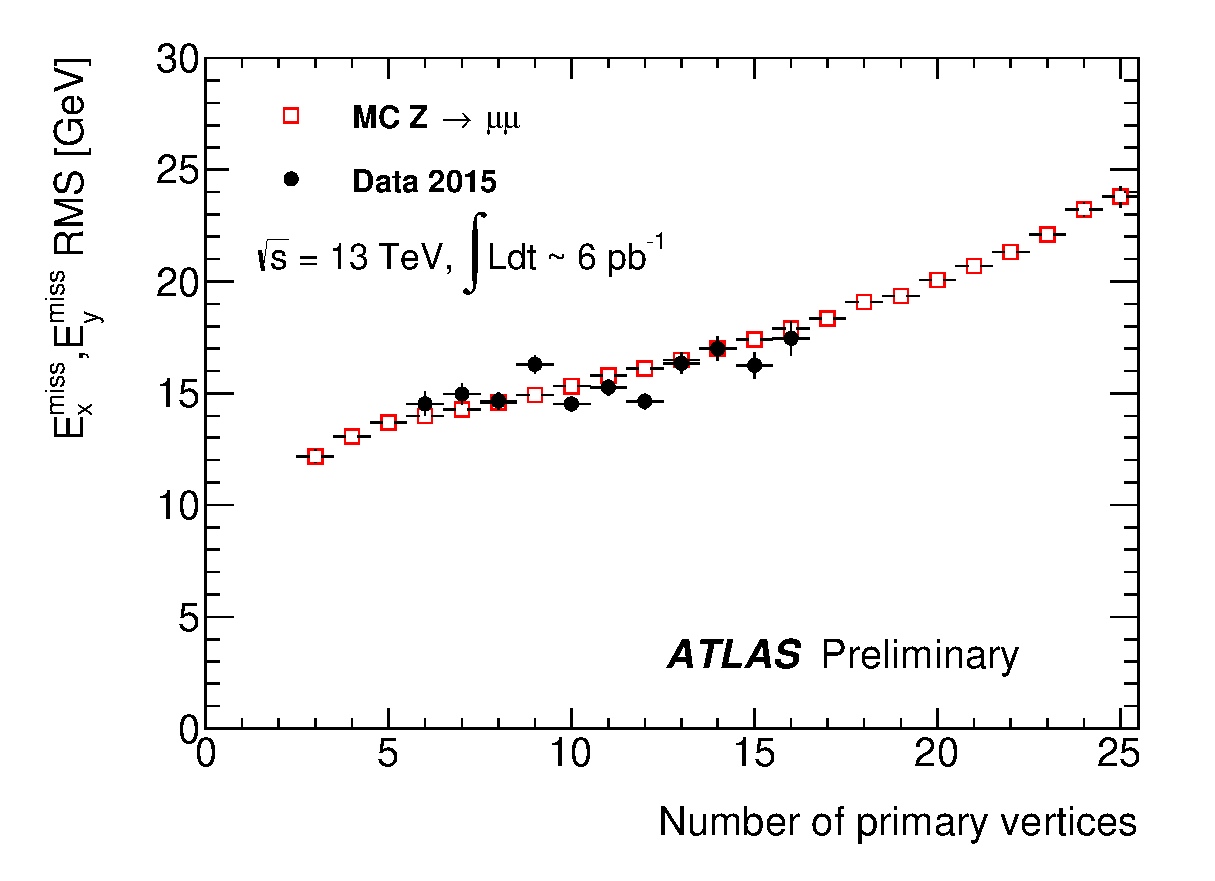
\includegraphics[width=0.45\textwidth]{figures/METCalib/METReso_nVtx.eps}\hspace{0.05\textwidth}
\end{center}
\caption{Distribution of the TST $\met$ resolution relative to the total $E_t$ of reconstructed objects in $Z\rightarrow \mu\mu$ events and Distribution of the TST $\met$ resolution relative to the number of reconstructed vertexes in $Z\rightarrow \mu\mu$ events.  $\met$ resolution degrades as $E_T$ and pileup increases.  (Figures taken from \cite{METReco})}
\label{fig:MET_reso} 
\end{figure}

%\indent Biases in the reconstructed $\met$ can be both in the form of direction.  The mean value of the reconstructed $\met$ projected onto the direction of flight of the $Z$ boson in the transverse plane ($A_Z$) is a useful quantity to describe any bias in the $\met$ soft term.  $Because the $Z\rightarrow \mu\mu$ do not contain true $\met$, an unbiased $\met$ would have an average of zero in the projection of the $\met$ onto the $Z$ direction.  \\

%\indent Distributions showing the bias on the reconstructed $\met$ in direction is shown in figure \ref{}.




